\section{Natural Language Generation}

Natural Language Generation (NLG) is a sub-field of Natural Language Processing that attempts to generate sequences of words that resemble natural human languages. Traditionally, this was done either by using production rules of a predefined grammar, or by performing statistical analyses of existing human-written texts to predict sequences of words, based on their occurrence probabilities \citep{cambria2014jumping}. Markov-chain text generators are an example of the latter, popularized by their usage in parody text generation \citep{jelinek1985markov}.

This broad classification of problems has multiple applications including, but not limited to:
\begin{itemize}
	\item Neural machine translation (NMT), in which the generation objective is to produce a semantically similar sentence in a target language, given a sentence in a source language \citep{bahdanau2014neural,cho2014properties,luong2015effective,wu2016google}.
	\item Dialogue generation, in which the objective is to produce a natural and syntactically correct response to a provided utterance \citep{cavazza2005dialogue,li2016persona,li2016deep,li2017adversarial}.
	\item Text summarization, which eliminates superfluous and non-pertinent information in a body of text, to express the idea using fewer words \citep{barzilay1999using,gong2001generic,conroy2001text}.
	\item Data-to-text report generation, which utilizes structured data, sourced from a relational data format, to fill out a text template \citep{goldberg1994using,reiter2007architecture,gatt2009data}.
\end{itemize}


\section{Multi-Layer Perceptrons}

Multi-layer perceptrons (MLP) are widely used in the neural network literature as the simplest vanilla artificial neural network. An MLP typically comprises one or more hidden layers that learn intermediate representations before producing an output layer. A simple MLP classification architecture for MNIST digits \citep{lecun2010mnist,deng2012mnist} is depicted in Figure \ref{fig:mlp-network}. The network is represented as a directed graph containing nodes and edges, where each node represents a neuron and each edge represents a learned weight. Each weight here is a model parameter. In this example, the weight between two successive layers are densely interconnected. Given a layer of $m$ nodes and a subsequent layer of $n$ nodes that are densely connected, we require $m*n$ edges (or weights) to connect the nodes of these two layers. These $m*n$ edges form a matrix representing the model parameters that transform a vector represented in the first layer to a vector represented in the second layer.

\begin{figure}[ht]
	\centering
	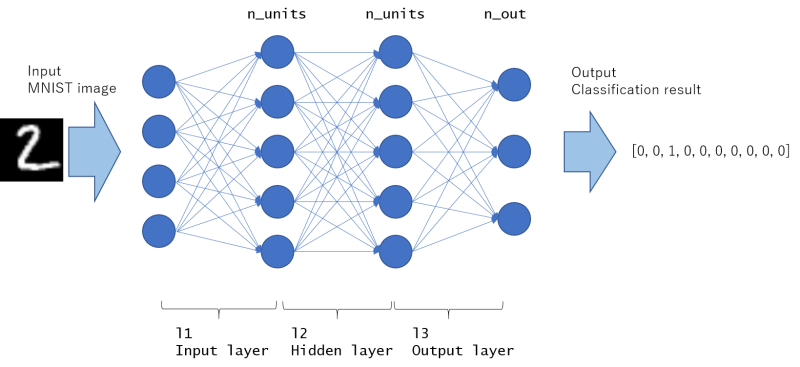
\includegraphics[width=\textwidth]{images/mlp-network}
	\imgsrc{\url{http://corochann.com/mnist-training-with-multi-layer-perceptron-1149.html}}
	\caption{\label{fig:mlp-network} Multi-Layer Perceptron}
\end{figure}

In terms of function approximation, a multilayer perceptron can be thought of as nested function calls on the input $x$. For example, assume that the intermediate layers approximate the functions $f_1$ and $f_2$, and the output layer approximates the function $f_3$ in the example presented in Figure \ref{fig:mlp-network}. We can then say that the relation of the output distribution $y$ with respect to the features in the input sample $x$ would be described as $y = f_3(f_2(f_1(x)))$. The back-propagation of the objective loss over the weights of the network is achieved by using the chain-rule to differentiate this nested function. The gradients thus obtained are then used to update the weights, thereby changing how the output layer is computed during the next iteration of computation through the directed graph \citep{lecun1989backpropagation}.

The activation functions applied at each layer could either be linear or non-linear. The most popularly used non-linear activation functions are sigmoid, tanh, ReLU etc., which are typically used in the intermediate layers of the network. In the case of multi-label prediction problems, the output layer is typically a softmax distribution over the possible output classes. The softmax activation is simply the binary logistic regression classifier that generalizes to multiple classes, since the output of the softmax function can be used to represent a categorical distribution (Equation \ref{eqn:softmax-function}).

\begin{equation} \label{eqn:softmax-function}
	P(y=j \mid \mathbf{x}) = \frac{e^{\mathbf{x}^\mathsf{T}\mathbf{w}_j}}{\sum_{k=1}^K e^{\mathbf{x}^\mathsf{T}\mathbf{w}_k}}
\end{equation}

An MLP classifier is trained by minimizing a cross-entropy loss between the predicted softmax distribution $y$ and the true distribution $y'$.
\begin{equation}
	\mathcal{H}_{y'} (y) := - \sum_{i}^K y_{i}' \log (y_i)
\end{equation}


\subsection{Dropout}

Dropout is a regularization technique used during the training of neural networks. It was proposed by \cite{srivastava2014dropout} as a simple method to prevent a model from over-fitting the approximately learned function on the training data. The idea of dropout is to randomly ignore a set of neural network weights i.e. randomly set function parameters to 0 during each instance of the forward pass, as shown in Figure \ref{fig:dropout}.

\begin{figure}[ht]
	\centering
	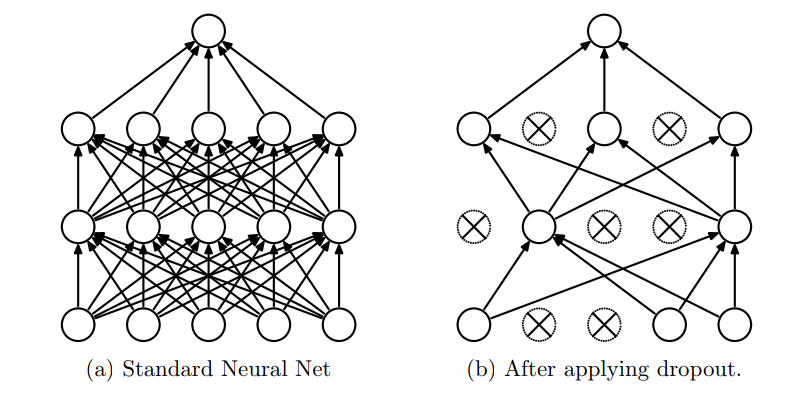
\includegraphics[width=\textwidth]{images/dropout}
	\imgsrc{\cite{srivastava2014dropout}}
	\caption{\label{fig:dropout} Dropout}
\end{figure}

Each neuron / unit is dropped out with a predefined probability, which can be viewed as a model hyperparameter. This allows for more generalized and robust functions being learned by minimizing the co-dependence of neurons on each other. Dropout has also been empirically shown to improve experiment results on several supervised learning tasks in vision, speech recognition, document classification and computational biology \citep{srivastava2014dropout}.


\section{Convolutional Neural Networks}

A convolutional neural network (CNN) \citep{lecun1995convolutional} is a specialized neural network that is optimized for feature extraction from local regions in data, for instance a specific object in an image, or a specific attribute in a body of text. Using densely connected multi-layer perceptrons for feature extraction from all the pixels of an image increases the number of parameters and slows down the training process. Instead, convolutional networks use shared weights over the source data that are called `filters'.

The `convolution' within a convolutional neural network is implemented using a filter. A filter is a learned function that transfers an arbitrary spatial representation of the image, say $3\text{px} * 3\text{px}$, into a single value and this is done for all the similar spatial zones in the image. 2-dimensional convolutions are used to process features in images and video because of their inherent spatial nature. A 1-dimensional equivalent could be used to extract features from contiguous regions of text, usually 3 to 5 words \citep{kim2014convolutional}. These features are then sub-sampled to reduce the dimensionality for subsequent layers. This is typically achieved by max-pooling or average-pooling, which simply requires aggregating all the spatially proximal region activations produced by the convolutional layer.

The strategy of stacking convolutional and pooling layers allows the network to learn parameters that are translation invariant. In simpler words, an object can be identified regardless of its location in an image, and an attribute can be identified regardless of its position in a body of text.

An example CNN architecture is presented in Figure \ref{fig:cnn}.

\begin{figure}[ht]
	\centering
	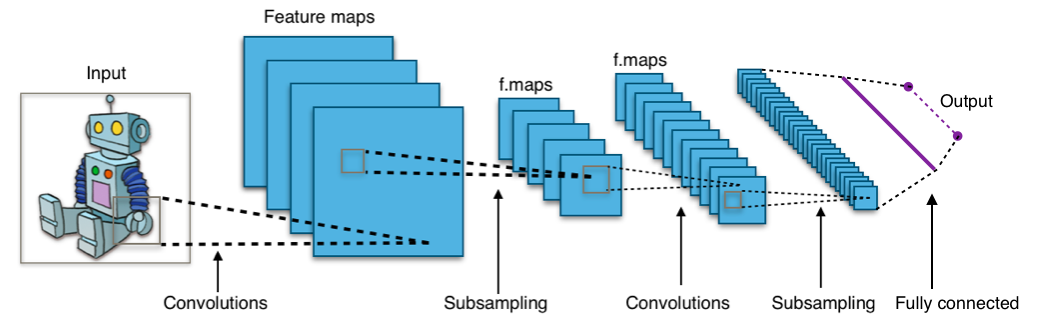
\includegraphics[width=\textwidth]{images/cnn}
	\imgsrc{\url{https://commons.wikimedia.org/wiki/File\%3ATypical_cnn.png}}
	\caption{\label{fig:cnn} Convolutional Neural Network}
\end{figure}

Since their inception, CNNs have been proven to achieve state-of-the-art results in multiple task settings within vision and language, especially with the use of deep convolutional architectures \citep{lawrence1997face,krizhevsky2012imagenet,karpathy2014large,kalchbrenner2014convolutional,kim2014convolutional,hu2014convolutional}.


\section{Recurrent Neural Networks}

Recurrent neural networks (RNNs) are a sub-class of artificial neural networks that are commonly used for sequence processing. Its units forms a directed graph that operates on a sequence of inputs in a temporally-distributed manner. This makes them a useful tool for extracting features from arbitrary length sequences of input like audio or text. The optimization problem an RNN tries to solve is to predict the next element in a sequence given the historical context, as shown in Equation \ref{eqn:rnn-next}.
\begin{equation} \label{eqn:rnn-next}
	P(w_1, \cdots, w_T) = \prod_{i=1}^T P(w_i | w_1, \cdots, w_{i-1})
\end{equation}

The language model is built in such a way that the features extracted from the sequence at time-step $t$ depend on the features observed during the time-steps $0 \cdots t-1$. A graphical depiction of a temporally-unrolled RNN is shown in Figure \ref{fig:recurrent-neural-network-unfold}.

\begin{figure}[ht]
	\centering
	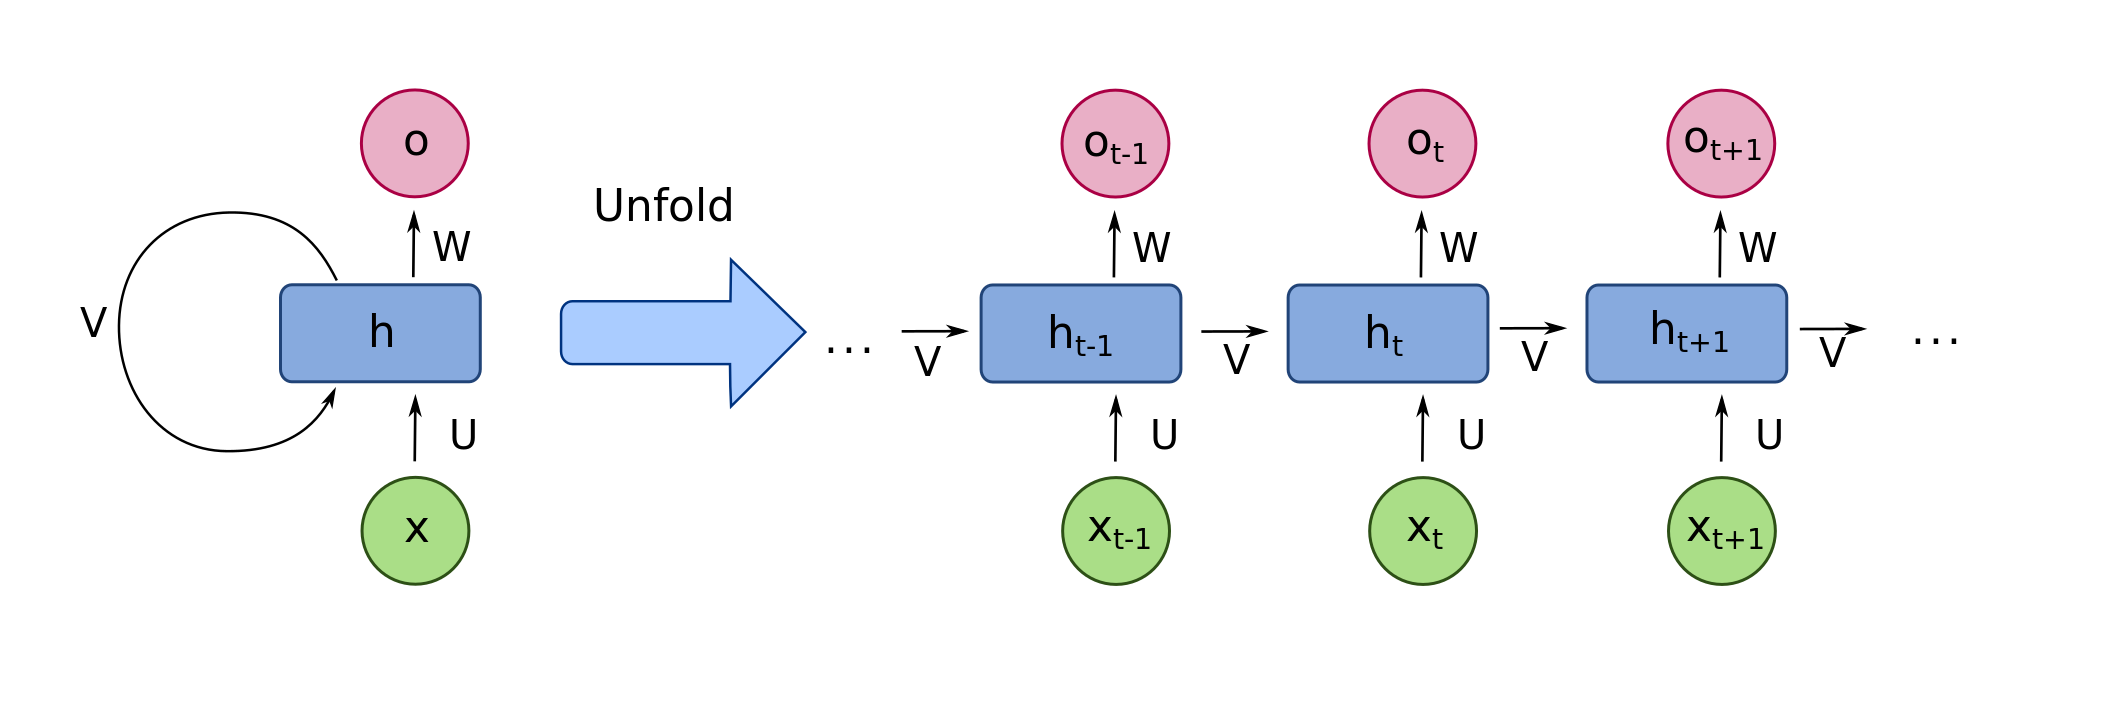
\includegraphics[width=\textwidth]{images/recurrent-neural-network-unfold}
	\imgsrc{\url{https://commons.wikimedia.org/wiki/File:Recurrent_neural_network_unfold.svg}}
	\caption{\label{fig:recurrent-neural-network-unfold} Recurrent Neural Network}
\end{figure}

The most recent and useful variants of recurrent units provide the ability to retain `memory' of the context in which the current features are to be extracted. In the domain of language processing, this typically implies that the recurrent unit has a stored memory of the previously observed words in a sequence, and this property grants it the ability to learn context as part of the feature space. The prominent variants of recurrent units used in neural networks to extract features from sequences using a memory mechanism, are Long Short-Term Memory (LSTM) units \citep{gers2001lstm} and Gated Recurrent Units (GRU) \citep{chung2014empirical}.

Recurrent networks in the domain of natural language processing are used frequently for both natural language understanding (NLU) tasks, as well natural language generation (NLG) tasks \citep{bengio2003neural,morin2005hierarchical,mikolov2010recurrent}. Similar to the manner in which recurrent networks can extract features from arbitrarily long sequences of vectorized text, they can also be used to produce text sequences from a unit vector representation of text, as represented in Figure \ref{fig:rnn-nmt}.

This is achieved by conditioning the generation of the first word of text either on some latent variable produced by a model, or by sampling from a generative distribution, and conditioning the generation of each subsequently predicted word on the word that was predicted in the previous time-step, until the model predicts an end-of-sentence (EOS) token.

\begin{figure}[ht]
	\centering
	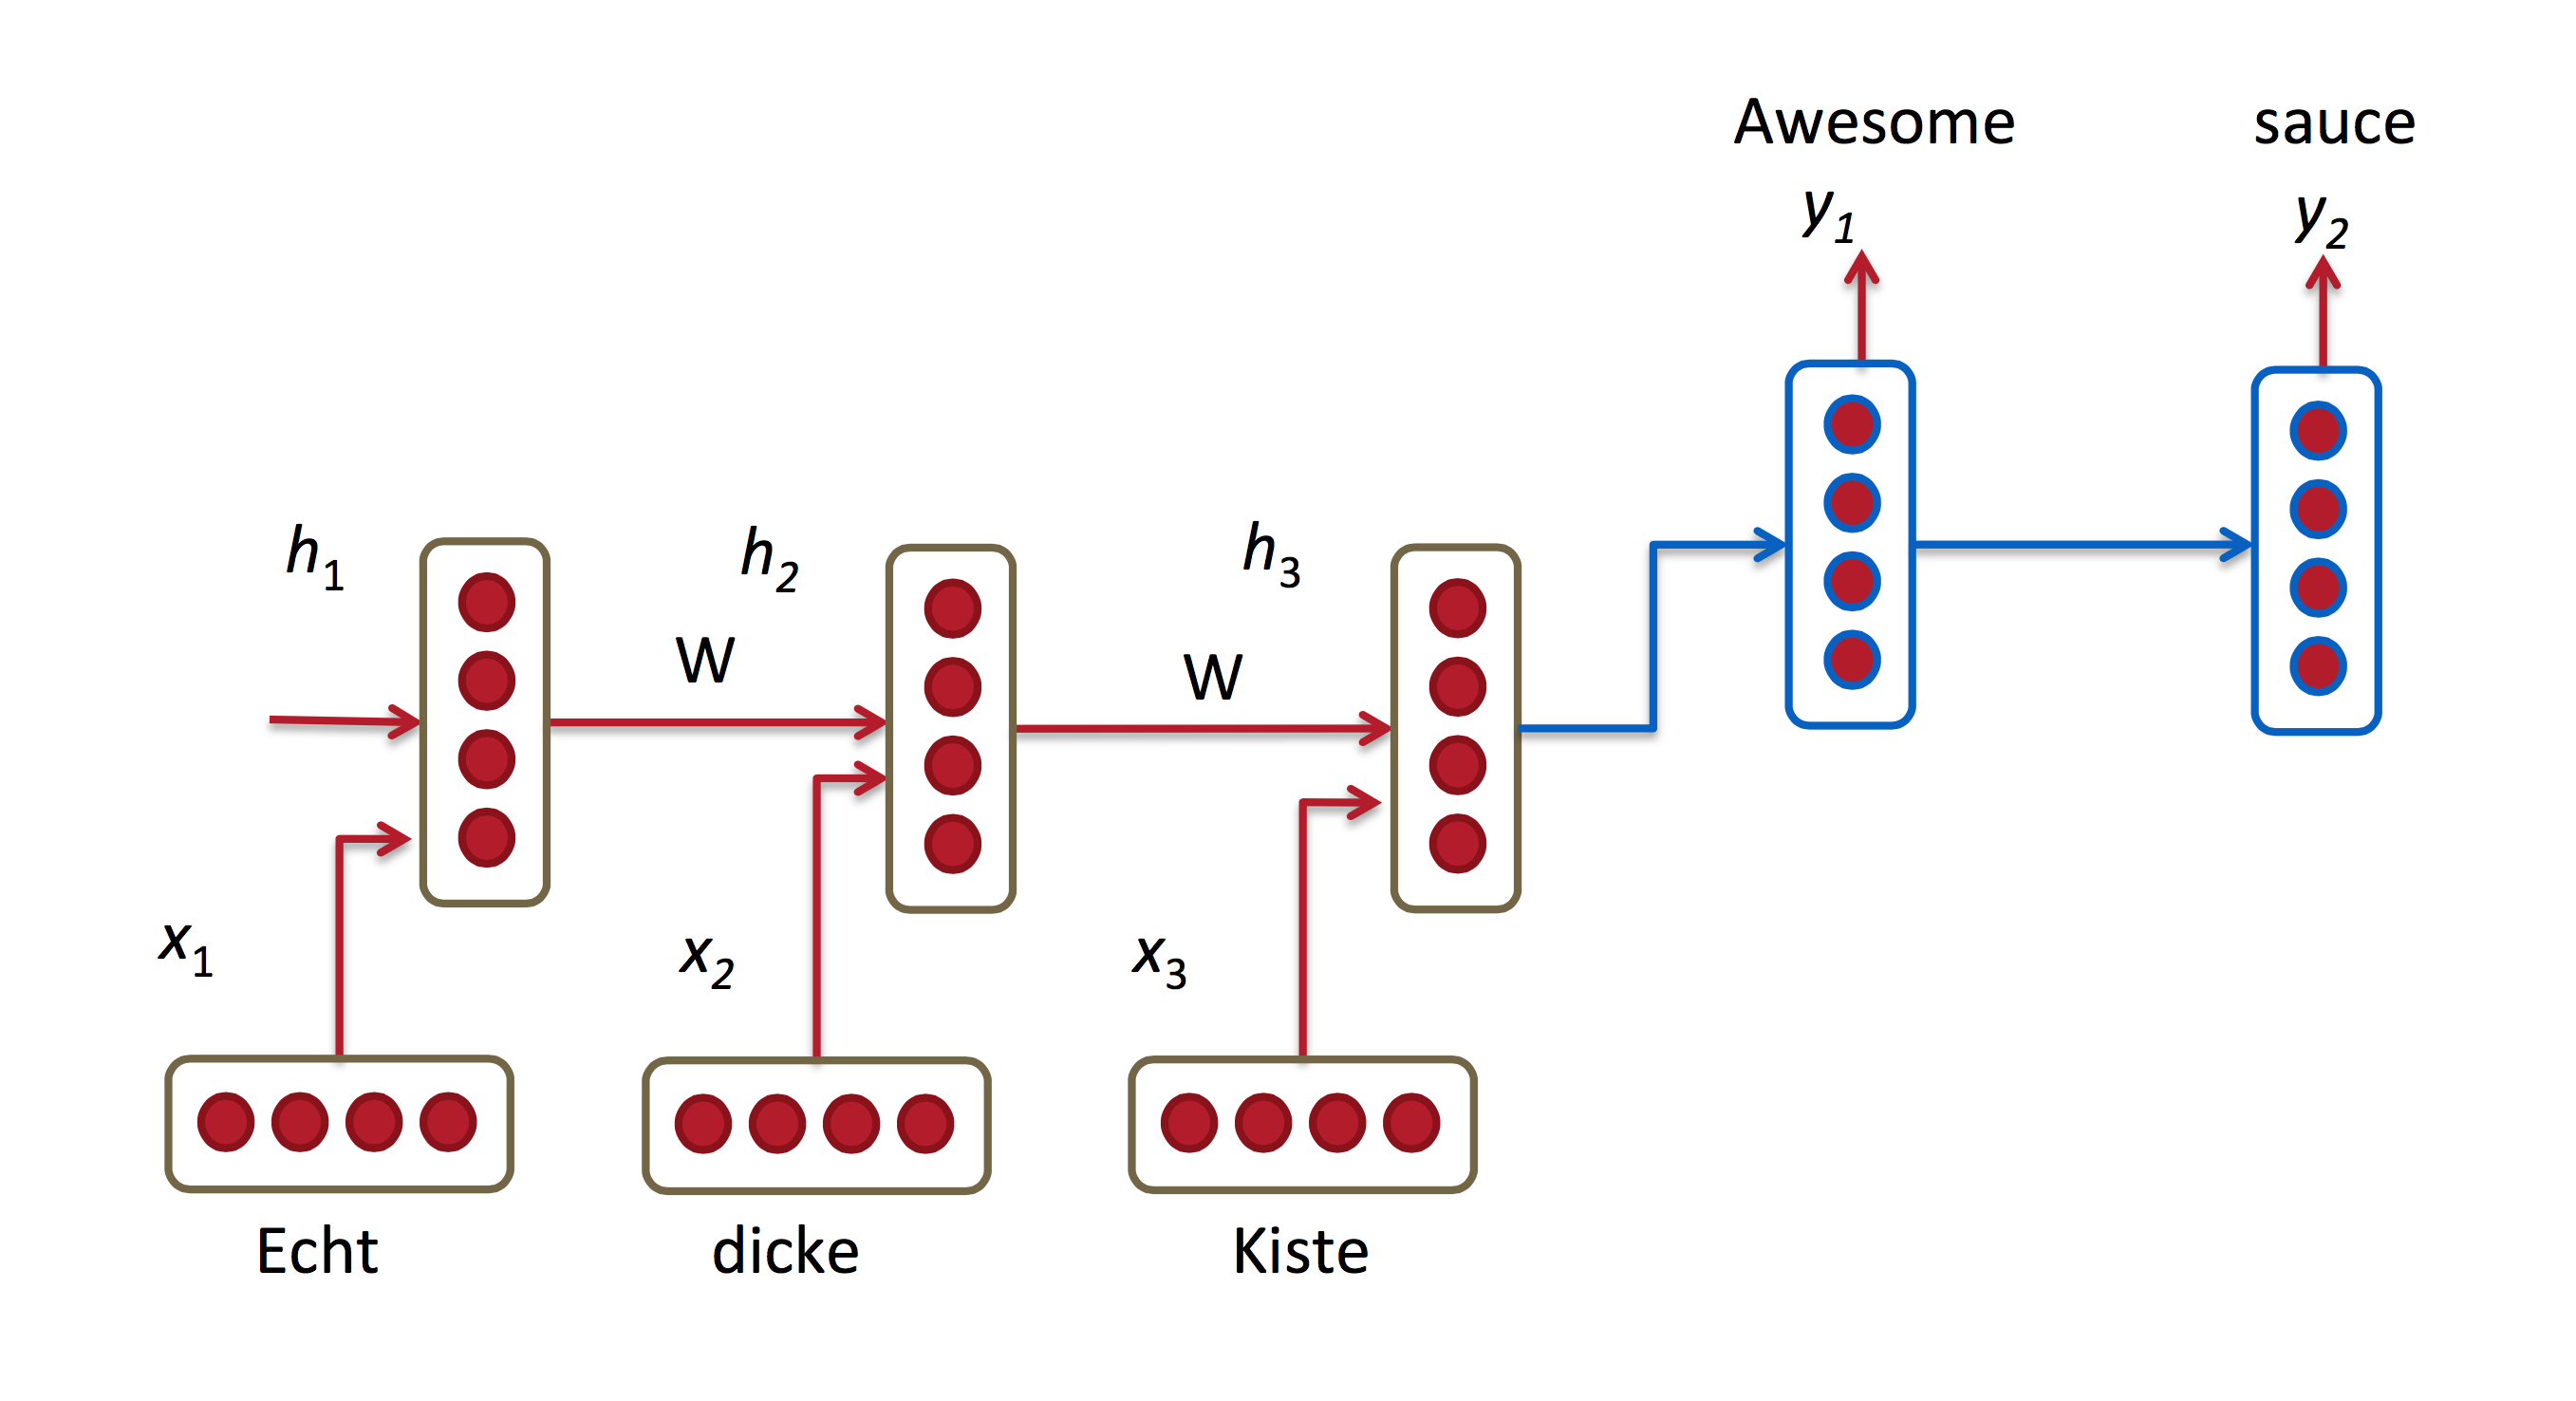
\includegraphics[width=\textwidth]{images/rnn-nmt}
	\imgsrc{\url{http://www.wildml.com/2015/09/recurrent-neural-networks-tutorial-part-1-introduction-to-rnns}}
	\caption{\label{fig:rnn-nmt} Recurrent Encoder-Decoder Model}
\end{figure}


\subsection{Long Short-Term Memory}

As described in the previous section, recurrent neural networks (RNN) learn representations of the data over temporal sequences, like text or audio features. However, in practice, RNNs don't seem to be able to assign priorities to which of the past data they choose to ascribe a higher importance to. This is detrimental to their usage in tasks that require processing of long sequences of data like in text, audio or video processing. This lack of ability to learn long-term dependencies in the input features is shown in previous work by \cite{bengio1994learning}.

Long Short-Term Memory (LSTM) units, as described first by \cite{hochreiter1997long}, seek to address this issue by explicitly modelling how much to retain and forget at each time-step during the RNN's training procedure.

\begin{figure}[ht]
	\centering
	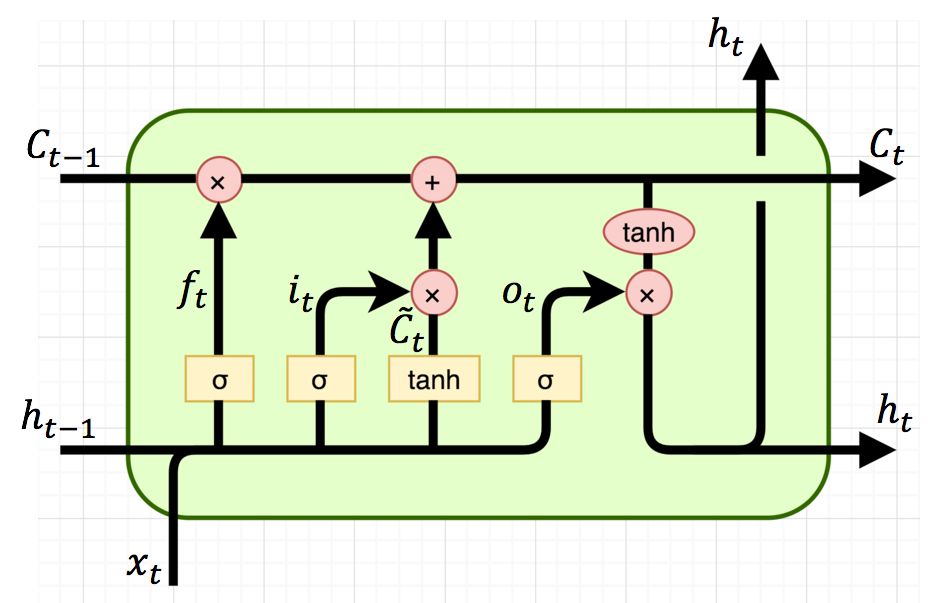
\includegraphics[width=\textwidth]{images/lstm}
	\imgsrc{\url{https://isaacchanghau.github.io/post/lstm-gru-formula}}
	\caption{\label{fig:lstm} Long Short-Term Memory Unit}
\end{figure}

The structure of an LSTM is depicted in Figure \ref{fig:lstm}. An LSTM is comprised of three distinct gating layers internally - namely the forget gate, input gate and output gate - that determine its outputs: the new cell state and hidden state. As can be seen in Figure \ref{fig:lstm}, the cell state $C_t$ passes through the LSTM mostly unperturbed, which is intended to address the problem of vanishing gradients \citep{hochreiter1999vanishing}.

The forget gate uses a sigmoid activation to squash the values of the output of the previous time-step between 0 and 1, which can be understood as semantically equivalent to deciding how much of the previous cell state to forget.
\begin{equation*}
	f_t = \sigma(W_f*[h_{t-1}, x_t] + b_f)
\end{equation*}

The input gate also uses a sigmoid activation on the previous hidden state, which is multiplied by the candidate cell state $\hat{C_t}$. The value thus obtained is then multiplied by the forget-gated previous cell state to form the next cell state.
\begin{align*}
	i_t =
	 & \sigma(W_i*[h_{t-1}, x_t] + b_i) \\
	\hat{C_t} =
	 & \tanh(W_c*[h_{t-1}, x_t] + b_c)  \\
	C_t =
	 & f_t * C_{t-1} + i_t * \hat{C_t}
\end{align*}

Now that we have obtained the cell state, we propagate that through to the next time-step. To obtain the hidden state, we use an output gate, again with a sigmoid activation, to gate the cell-state and create the hidden-state for the next time-step.
\begin{align*}
	o_t =
	 & \sigma(W_o*[h_{t-1}, x_t] + b_o) \\
	h_t =
	 & \tanh(C_t)
\end{align*}

The efficacy of LSTM-backed RNNs is evident from the prevalence of their usage in language modelling literature \citep{sundermeyer2012lstm,gers2001lstm,graves2005framewise} \footnote{\url{https://karpathy.github.io/2015/05/21/rnn-effectiveness}}.

\subsection{Gated Recurrent Units}

Gated Recurrent Units (GRU) \citep{cho2014learning} are similar to LSTMs in that they possess gating mechanisms to assist with long-term dependency learning. They differ from LSTMs in a few aspects, like the merging of the input and forget gates into a single update gate. They also merge cell state and hidden state, emitting only a single output vector after the computations within the cell. Figure \ref{fig:gru} depicts the internal GRU states and gates.

\begin{figure}[ht]
	\centering
	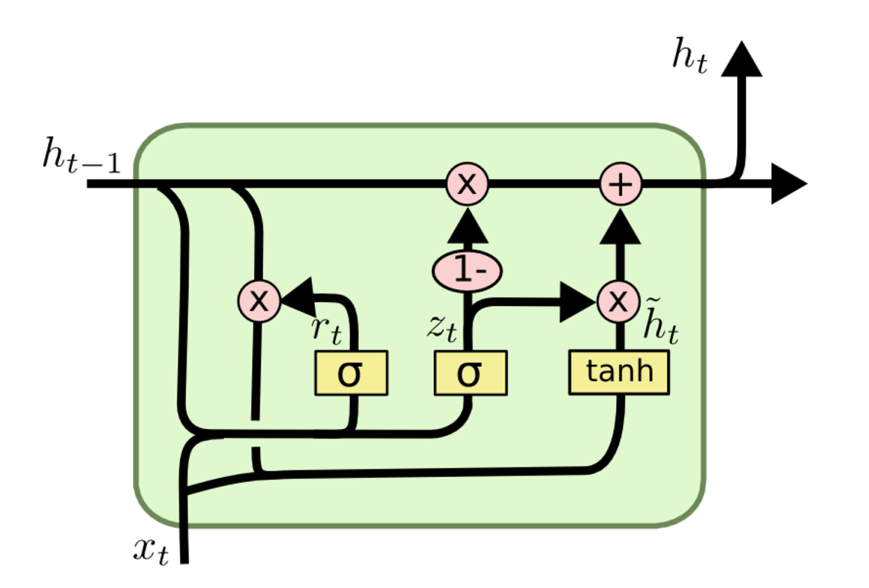
\includegraphics[width=\textwidth]{images/gru}
	\imgsrc{\url{https://isaacchanghau.github.io/post/lstm-gru-formula}}
	\caption{\label{fig:gru} Gated Recurrent Unit}
\end{figure}

GRUs are a lot simpler to work with in practice due to their having only a single output. They have been used interchangeably with LSTMs as memory units for recurrent neural networks \citep{chung2015gated,fu2017style}.


\section{Autoencoders}

Autoencoders are models that are parameterized to convert arbitrary data into a latent representation (encoder), and recover the original data back from the latent representation (decoder). In this setup, the dimensionality of the latent representation is usually much smaller than that of the actual data. A simple autoencoder architecture is depicted in Figure \ref{fig:autoencoder-structure}.

\begin{figure}[ht]
	\centering
	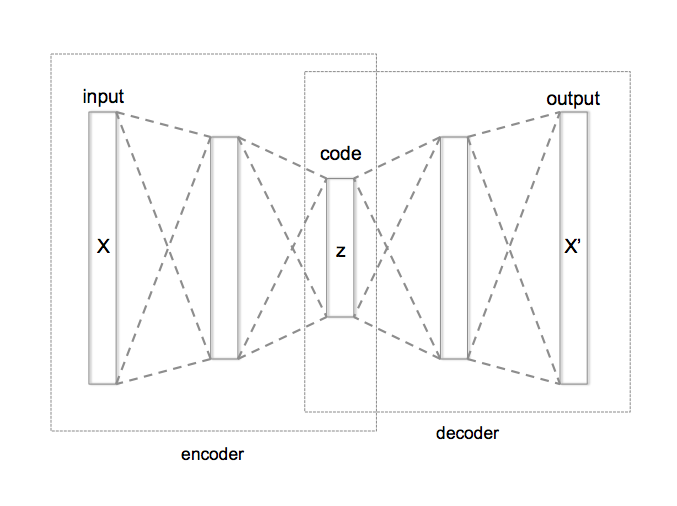
\includegraphics[width=\textwidth]{images/autoencoder-structure}
	\imgsrc{\url{http://mlexplained.com/2017/12/28/an-intuitive-explanation-of-variational-autoencoders-vaes-part-1}}
	\caption{\label{fig:autoencoder-structure} Model Architecture: Autoencoder}
\end{figure}

By training a model to reconstruct data that is funnelled through a lower dimensional representation, two objectives can be achieved simultaneously:
\begin{itemize}
	\item The encoder weights of the model could be used to extract the most salient features of the data in a compressed representation, which is a better input feature format for downstream processing or learning algorithms. \citep{hinton2006reducing}
	\item The decoder weights of the model could be used as a generator. Given that we can sample from the distribution of the existing latent representations learned, or from a predefined prior (in a variational autoencoder), we can generate plausible novel data.
\end{itemize}

In the context of natural language, the encoder can be utilized as a sentence-encoding feature-extractor and the decoder can be utilized as a generative model. Autoencoders are also able to de-noise data given pairs of noisy and regular data, by learning a de-noising function, which can then be used for actual noisy data. These properties make autoencoders a good framework to utilize to implement sequence-to-sequence models, wherein both the encoder and decoder weights of the model are parameterized by neural networks that process and generate sequences of data, respectively.

\subsection{Variational Autoencoders}

Variational autoencoders (VAEs) \citep{kingma2013auto} are a probabilistic variant of autoencoders. The general structure of a VAE is the same as that of a deterministic autoencoder, with an encoder that learns a compressed latent space and a decoder that learns a function to map the latent space into the original data. In contrast with the deterministic autoencoder, a variational autoencoder parameterizes representations of the latent mean and variance as separate spaces. The method of variational inference requires placing conjugate priors on the mean and variance of the hitherto unknown latent representation. The encoder is then trained to learn the approximate posterior distribution, and the decoder is trained to generate novel data using samples taken from the prior distribution. The family of distributions used for this purpose are Gaussian. A simple VAE architecture is depicted in Figure \ref{fig:vae-structure}.

\begin{figure}[ht]
	\centering
	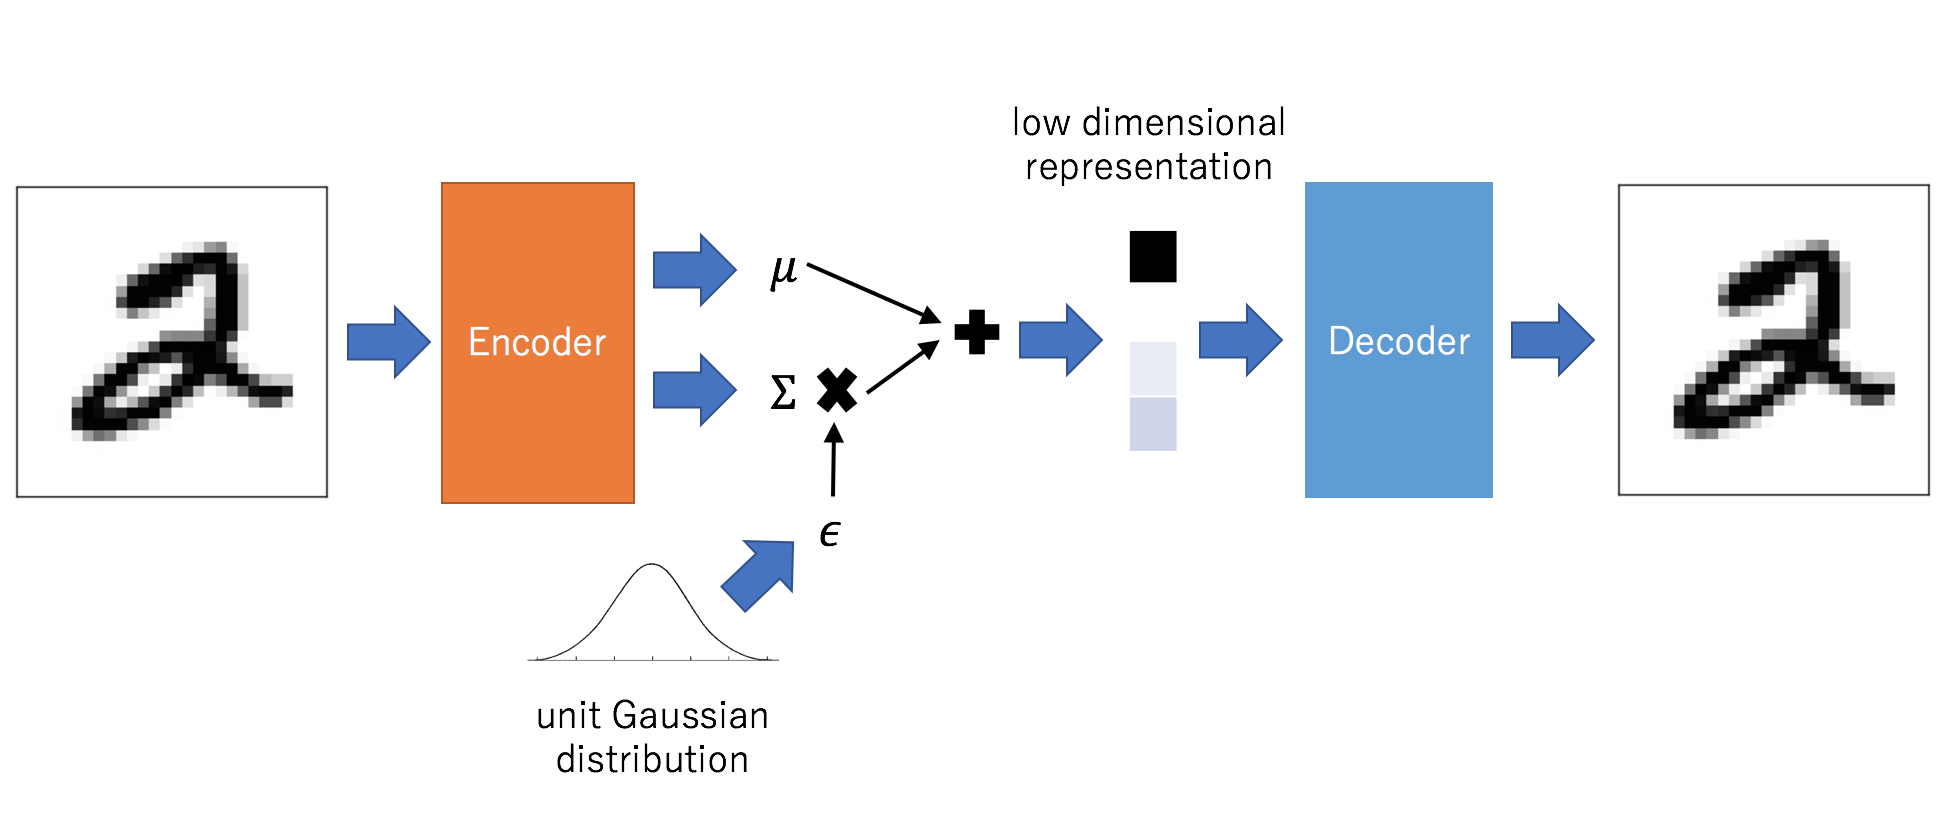
\includegraphics[width=\textwidth]{images/vae-structure}
	\imgsrc{\url{http://mlexplained.com/2017/12/28/an-intuitive-explanation-of-variational-autoencoders-vaes-part-1}}
	\caption{\label{fig:vae-structure} Model Architecture: Variational Autoencoder}
\end{figure}

In addition to the reconstruction loss that a deterministic autoencoder uses, a metric of distance is used to evaluate how closely the learned representations of mean and variance resemble a Gaussian distribution with mean 0 and unit variance. The Kullback-Leibler (KL) divergence \citep{kullback1951information} is used to penalize learned representations that do not resemble the prior. However, we cannot compute the KL divergence directly. Instead we compute an alternative objective that is equivalent to the KL divergence up until an added constant. This is called the evidence lower-bound (ELBO). The ELBO objective maximized in a variational autoencoder model is given in Equation \ref{eqn:elbo}:
\begin{equation} \label{eqn:elbo}
	ELBO(q) = \mathbb{E}_{q(z)} [(\log(p(x|z))] - \mathbb{KL}(q(z)||p(z))
\end{equation}

Simultaneously, for the decoding step, we sample from the prior, utilizing the re-parameterization trick to ensure that the model remains differentiable. As a result, the decoder is trained as a generative network that can randomly sample from the prior and generates plausible data that is similar to the input distribution. The decoder being able to act as a generative model independently is what sets a VAE apart from a deterministic autoencoder.


\section{Word Embeddings}

Prior to the usage of matrix factorization and neural models to learn continuous word representations, the numerical representations used for words and documents were one-hot representations, word-ngrams \citep{brown1992class} or tf-idf weighted statistics. Word-ngrams are useful for expressing probability distributions of word occurrences in a corpus. Higher order ngrams (bigrams, trigrams, four-grams etc.) also take into account the context of nearby words, and can be used to construct language models.

However, these methods use discrete word or character occurrence counts to represent words and documents, and these representations scale with the size of the input corpus vocabulary for word-based models. This makes discrete word representation based language models computationally inefficient for large corpora with diverse vocabularies. Character-based models, on the other hand, are liable to produce invalid words and don't work as well with recurrent memory units as words do \citep{bojanowski2015alternative}. These methods are also ineffective at modelling semantic inter-word relationships.

Word2Vec, which aims to alleviate these problems, is a vector space model that embeds words into a continuous space. Also, semantically similar words in Word2Vec are embedded in nearby spaces \citep{mikolov2013distributed,mikolov2013linguistic,le2014distributed}. Word2Vec can model the corpus vocabulary in two different ways, namely CBOW and Skip-gram. The CBOW model predicts a target word from context words, whereas the Skip-gram model does the opposite and predicts target words from a single context word. Both model types are shown in Figure \ref{fig:efficient-models}

\begin{figure}[ht]
	\centering
	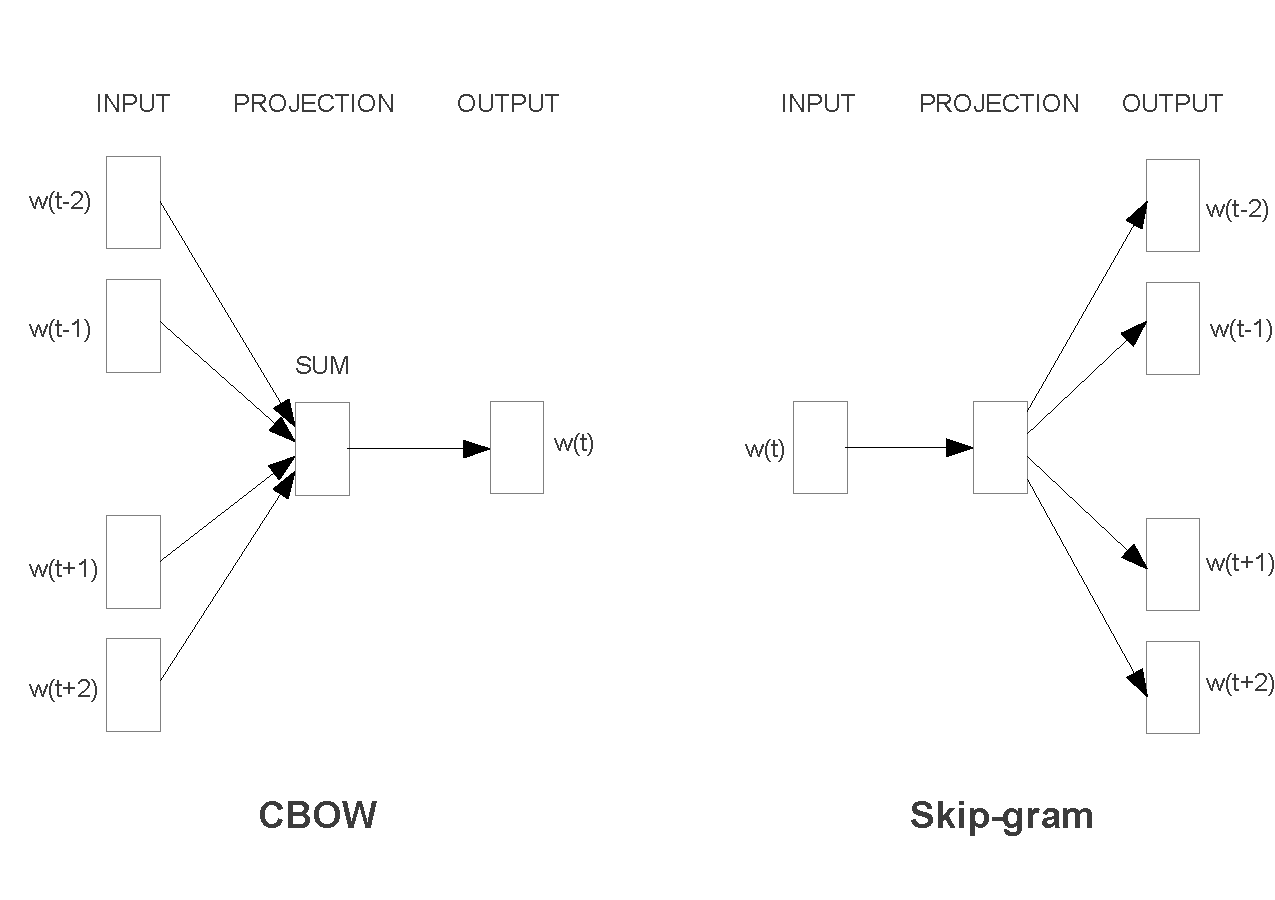
\includegraphics[width=\textwidth]{images/efficient-models}
	\imgsrc{\cite{mikolov2013efficient}}
	\caption{\label{fig:efficient-models} Word2Vec Model}
\end{figure}

The Word2Vec model is a simple shallow neural network, with single input, hidden and output layers. The hidden layer is of arbitrary size, called the embedding size. The embedding size is usually much lower that the vocabulary size, which is reminiscent of an autoencoder that learns a compressed salient representation of the words. The one-hot encoded input is transformed into its context or target word, depending on whether the algorithm chosen is CBOW or Skip-gram. This transformation is parameterized by the shallow neural network. After the model converges, the network weights connecting the input and the hidden layer can be used as parameters to obtain dense, continuous representations of words.

A surprising outcome of this embedding model is that translations within the learned vector space seem to emulate semantic (gender, tense) as well as factual relationships (country-capital), as shown in Figure \ref{fig:word2vec-linear-relationships}.

\begin{figure}[ht]
	\centering
	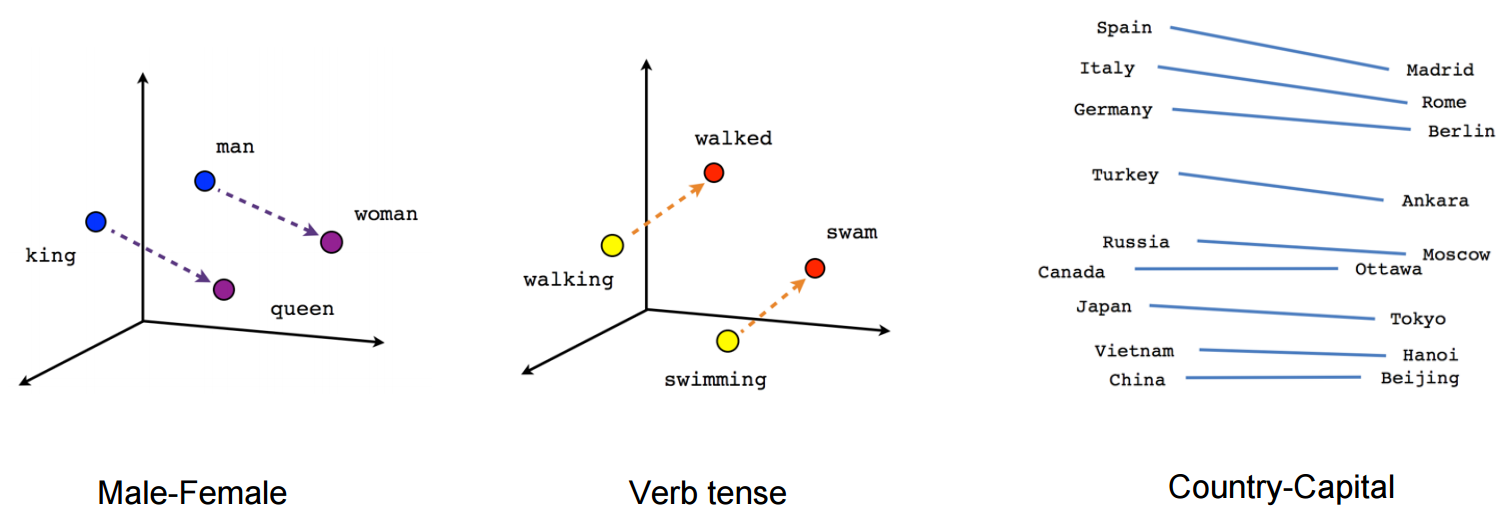
\includegraphics[width=\textwidth]{images/word2vec-linear-relationships}
	\imgsrc{\url{https://www.tensorflow.org/tutorials/word2vec}}
	\caption{\label{fig:word2vec-linear-relationships} Word2Vec Relationships}
\end{figure}

Word embedding neural models are also shown to be implicitly factorizing a word-context matrix by subsequent work in this area \citep{levy2014neural}.


\section{Sequence-to-Sequence Modelling}

Also abbreviated in the literature as Seq2Seq, this is a class of models that learns functions to transform one sequence into another. First introduced by \cite{sutskever2014sequence}, Seq2Seq is flexible framework for modelling transformations made to arbitrary length sequences, typically using a neural encoder-decoder framework. In the field of natural language processing, the main tasks that benefit from such an encoder-decoder framework are those for which there exists two distinct distributions of text, and the model is trained to learn the mapping from one to the other.

\cite{sutskever2014sequence} define a sequence-to-sequence model that learns a function (Equation \ref{eqn:seq2seq}) to map a sequence of inputs $x_1, \cdots , x_T$ to a sequence of outputs $y_1, \cdots , y_{T'}$, where the initial state $h$ is set to the hidden LSTM representation of $x_1, \cdots , x_T$.

\begin{equation} \label{eqn:seq2seq}
	p(y_1, \cdots , y_{T'} | x_1, \cdots , x_T) =	\prod_{t=1}^T p(y_t | h, y_1, \cdots , y_{t-1})
\end{equation}

This makes the Seq2Seq model an ideal framework using which one can implement solutions to several natural language generation tasks like neural machine translation, dialogue generation, text summarization, etc.

\section{Generative Adversarial Networks}

\cite{goodfellow2014generative} presented a novel generative model that utilizes the idea of a game-theoretic competition between a generative model which is a decoder, and a discriminative model which is a classifier. The general idea is to train the discriminate model, also known as the adversary, to be able to discriminate between the synthetic distribution that the generator model produces, and a true distribution that the generator trying to mimic. Figure \ref{fig:gans} depicts a sample GAN model architecture.

\begin{figure}[ht]
	\centering
	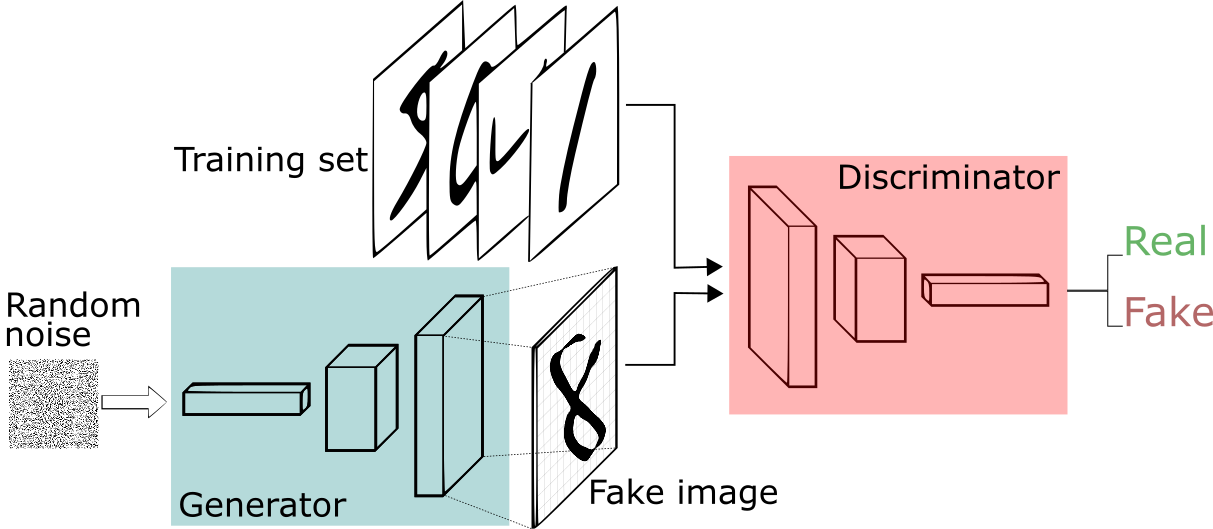
\includegraphics[width=\textwidth]{images/gans}
	\imgsrc{\url{https://deeplearning4j.org/generative-adversarial-network}}
	\caption{\label{fig:gans} Model Architecture: Generative Adversarial Networks}
\end{figure}

In the original formulation of adversarial training, which involves using a binary classifier, the generator learns weights to map a randomly initialized latent variable $z$ to a data distribution $x$ that it is unaware of. The discriminator is trained using the true distribution and samples generated by the generative model, with the objective to discriminate the true samples from the generated samples. The generator on the other hand, attempts to maximize the discriminator's classification error without directly modifying the discriminator's parameters, thereby producing plausible samples that mimic the true distribution. In this manner, both the generator and discriminator are simultaneously trained to both produce better synthetic samples, as well as differentiate between real and synthetic samples respectively. This min-max game is represented by Equation \ref{eqn:gan-minimaxgame}, where $D$ is the discriminator, $G$ is the generator and $V$ is the value-function or loss-function of the generative model.

\begin{equation}
	\label{eqn:gan-minimaxgame}
	\min_G \max_D V(D, G) = \mathbb{E}_{\bm{x} \sim p_{\text{data}}(\bm{x})}[\log D(\bm{x})] + \mathbb{E}_{\bm{z} \sim p_{\bm{z}}(\bm{z})}[\log (1 - D(G(\bm{z})))].
\end{equation}

This property the generator model's parameters possess - of translating random noise into plausible data samples - is used in areas of research within computer vision and natural language processing to produce novel data samples. Also, adversarial learning as a principle is an effective tool to ensure that a feature space is devoid of any arbitrarily chosen set of known attributes. We use this property of adversarial learning in our model to assist with the disentanglement of stylistic attributes.


\section{Visual Style Transfer}

The idea of neural style transfer was originally proposed by \cite{gatys2016image}. In the task described in the paper, the authors use two distinct images as input. The first image contributes the content, and the second contributes the style. The objective is to generate a final image that contains all of the physical objects visible in the first image, but depicted in the style (hue, brush strokes, texture, etc.) visible in the second.

\begin{figure}[ht]
	\centering
	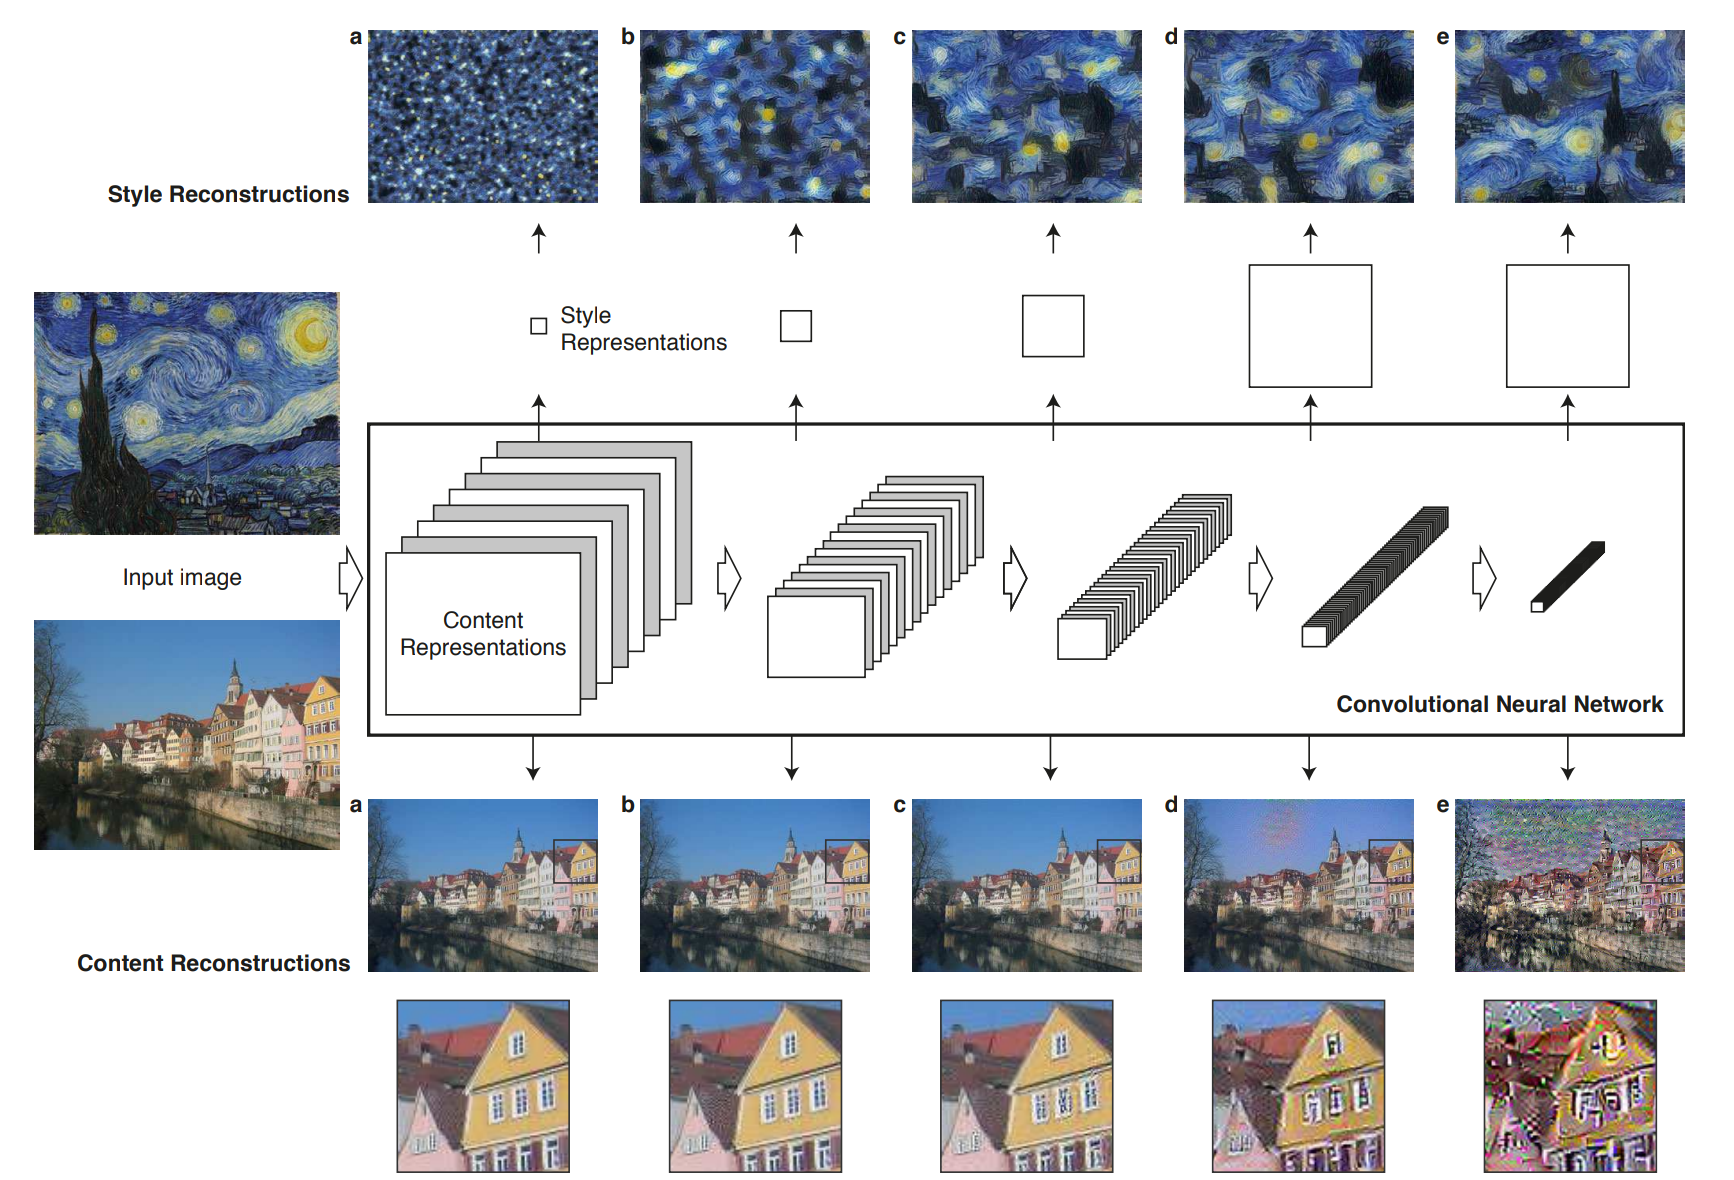
\includegraphics[width=\textwidth]{images/image-style-transfer}
	\imgsrc{\cite{gatys2016image}}
	\caption{\label{fig:image-style-transfer} Artistic Style Transfer in Images}
\end{figure}

The features, as with most of the state-of-the-art image processing techniques, are extracted from the images using Convolutional Neural Networks (CNNs) \citep{lecun1998gradient}, the deep neural network variants of which have been widely successful at image recognition tasks such as object recognition in the ImageNet dataset \citep{krizhevsky2012imagenet}.

As depicted in Figure \ref{fig:image-style-transfer}, subsequent layers of the CNN learn incrementally higher level features in both the style image and the content image. These learned features for the style and content images are stored for future use. To generate the final image, the authors begin with a random white noise image. This image is passed through both networks, the parameters of which extract both its style features and its content features.

This model uses two training objectives:
\begin{itemize}
	\item Minimize the the element-wise mean squared difference between the style features computed for the style image and the white-noise image.
	\item Minimize the the mean squared difference between the content features of the content image and the white noise image.
\end{itemize}

The overall training loss is a linear combination of the above objectives, and is used to iteratively modify the white-noise image until it has the style features of the style image and the content features of the content image.


In this chapter, we discussed the background needed to understand the methods used in our research and other related work. The next chapter builds on the fundamentals established here, and discusses previous attempts at neural disentanglement in the context of linguistic style transfer, as well as methods that do not use disentanglement as the basis of their style transfer model.
